\documentclass{beamer}
\usepackage[utf8]{inputenc}
\usepackage[T1]{fontenc}
\usepackage{lmodern}
\usepackage{amsmath}
\usepackage{tikz}
\usetikzlibrary{snakes}
\usepackage{xcolor} % Farben
\usepackage{fancyvrb} % Code
\usepackage[absolute,overlay]{textpos} % Bilder irgendwohin
\usepackage{bm} % Fett in Mathemodus
\usepackage{siunitx} % Einheiten
\usepackage{multicol} % Equations nebeneinander
\usepackage{algorithm2e} % Algorithmen
\usepackage{array} % Tabellenspalten zentriert
\usepackage{hyperref} % Links
\usepackage{ngerman}[babel]
\usepackage{calligra}
\usepackage[style=numeric]{biblatex}
\addbibresource{bib.bib}

\newcommand{\setfont}[2]{{\fontfamily{#1}\selectfont #2}}

\setbeamertemplate{bibliography item}{\insertbiblabel}
\setbeamercolor{bibliography entry note}{fg=black}

\usecolortheme{seahorse}
\definecolor{dark}{rgb}{0, 0.1, 0.3}
\definecolor{light}{rgb}{0.9, 0.933, 1}
\definecolor{fpga}{rgb}{0.8, 0.5, 0.9}
\setbeamercolor{normal text}{fg=black}
\setbeamercolor{structure}{fg=dark}
\setbeamercolor{footline}{fg=black}
\setbeamercolor{frametitle}{fg=light,bg=dark}
\setbeamertemplate{itemize items}[circle]
\beamertemplatenavigationsymbolsempty
\addtobeamertemplate{navigation symbols}{}{
    \usebeamerfont{footline}
    \usebeamercolor[fg]{footline}
    {\footnotesize \insertframenumber\\\vspace{0.15cm}}
}
\setbeamertemplate{title page}{
    \begin{center}
    Projektgruppe FastSense\\\vspace{0.2cm}
    \begin{LARGE}
    Meilenstein 2\\\vspace{0.2cm}
    Hardware Accelerated TSDF SLAM
    \end{LARGE}\\\vspace{0.5cm}
    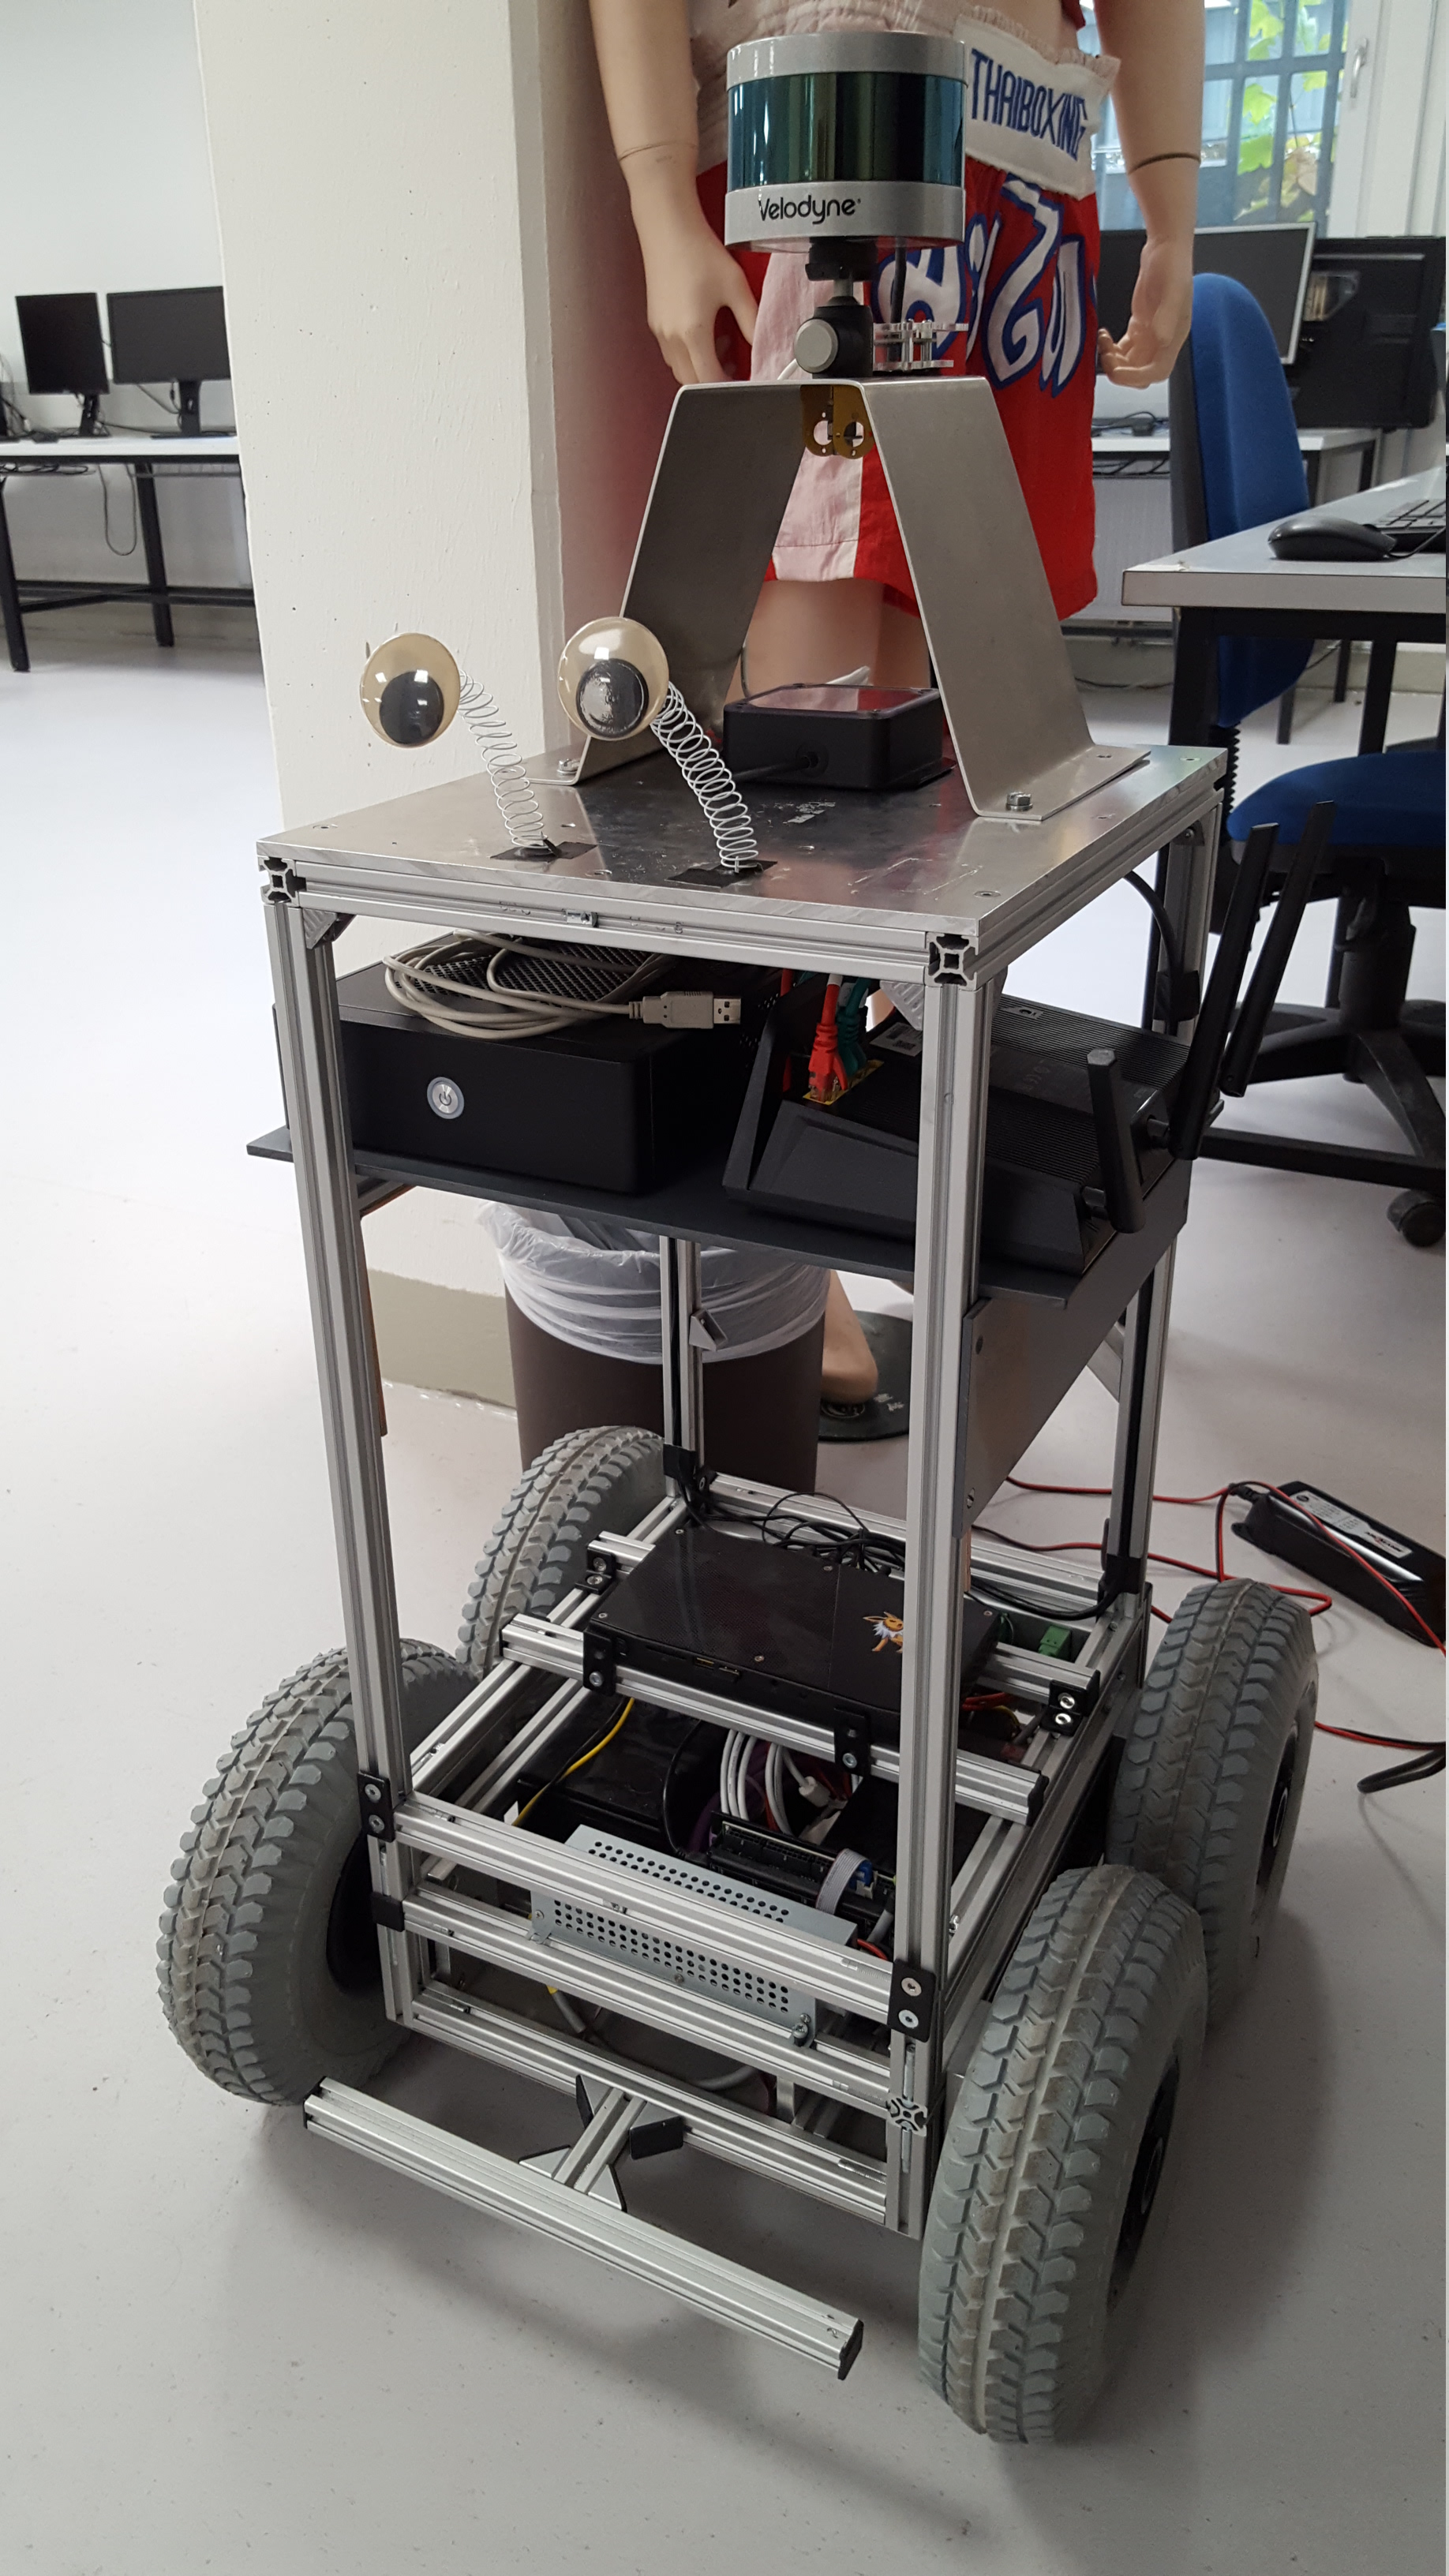
\includegraphics[height=5cm]{images/robot.jpg}\\\vspace{0.5cm}
    28. Oktober 2020
    \end{center}
}

\begin{document}

{\setbeamertemplate{navigation symbols}{}
%\usebackgroundtemplate{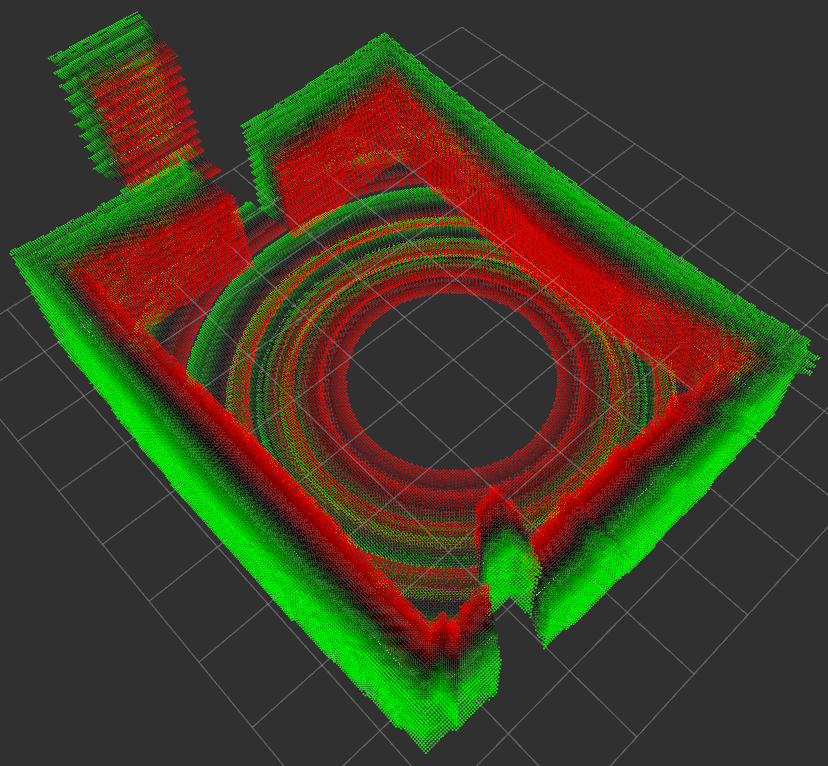
\includegraphics[width=\paperwidth]{images/tsdf_map.png}}
\begin{frame}
\titlepage
\end{frame}}

\begin{frame}
\frametitle{Inhalt}
\tableofcontents
\begin{textblock*}{1cm}(0cm,2cm)
\begin{tikzpicture}
\draw [white] (0, 2.64) rectangle +(1, 1);
\draw [light, ultra thick] (1, 0) -- (7, 0);
\node [right, dark] at (7, 0) {Live Demonstration};
\end{tikzpicture}
\end{textblock*}
\end{frame}



\section{Ziele und Anforderungen}
\begin{frame}{}
\begin{center}

\begin{tikzpicture}
\fill[light] (0, 0) rectangle (8, 2);
\node[dark] at (4, 1) {\begin{LARGE}\secname\end{LARGE}};
\end{tikzpicture}
\end{center}
\end{frame}

\subsection{Ziele für MS2}
\begin{frame}{\subsecname}
\begin{itemize}
\item Implementation von inkrementellem TSDF SLAM in \glqq{}autarker\grqq{} Box
\item Vorimplementation in Software
\item Implementation einzelner Komponenten in Hardware
\item Speicherung von Pose-Graph und TSDF-Karte
\item Evaluation durch Zeit- und Strommessung
\end{itemize}
\end{frame}

\subsection{Funktionale Anforderungen}
\begin{frame}{\subsecname}
\begin{itemize}
\item{Lokale TSDF-Map ausgeben}
\item{Aktuelle 6D-Pose ausgeben}
\item{Map auf Basis der IMU und Velodyne-Daten}
\item{Trajektorie und TDSF-Map für jede Pose speichern}
\item{Parameter zur Laufzeit anpassbar}
\end{itemize}
\begin{center}
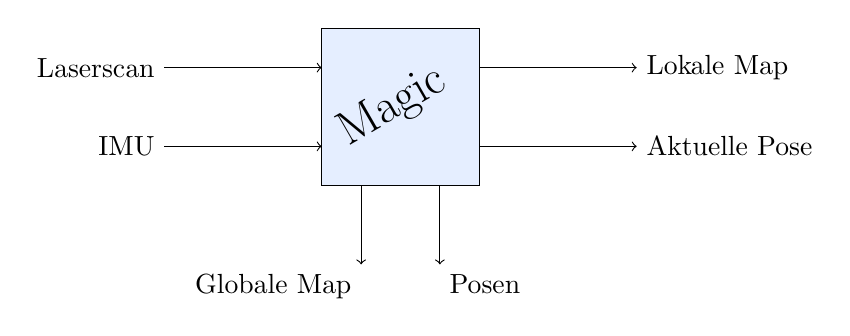
\begin{tikzpicture}
\draw [fill=light] (-1, -1) rectangle +(2, 2);
\node [rotate=30] at (-0.1, 0) {\LARGE\setfont{calligra}{Magic}};
\draw [->] (-3, 0.5) node [left] {Laserscan} -- (-1, 0.5);
\draw [->] (-3, -0.5) node [left] {IMU} -- (-1, -0.5);
\draw [->] (1, 0.5) -- (3, 0.5) node [right] {Lokale Map};
\draw [->] (1, -0.5) -- (3, -0.5) node [right] {Aktuelle Pose};
\draw [->] (-0.5, -1) -- (-0.5, -2) node [below left] {Globale Map};
\draw [->] (0.5, -1) -- (0.5, -2) node [below right] {Posen};
\end{tikzpicture}
\end{center}
\end{frame}

\subsection{Nicht-Funktionale Anforderungen}
\begin{frame}{\subsecname}
\begin{itemize}
\item{HW-Plattform: Trenz-Board}
\item{Entwicklungsplattform: Vitis}
\item{Beschleunigung der Algorithmen durch FPGA}
\item{Sensoren direkt am Board}
\item{Unit-Tests}
\item{Testbench}
\begin{itemize}
\item{Integration, Strommessung, Zeitmessung, Visualisierung}
\end{itemize}
\item{Logging}
\end{itemize}
\end{frame}



\section{Implementierung}
\begin{frame}{}
\begin{center}

\begin{tikzpicture}
\fill[light] (0, 0) rectangle (8, 2);
\node[dark] at (4, 1) {\begin{LARGE}\secname\end{LARGE}};
\end{tikzpicture}
\end{center}
\end{frame}

\subsection{Recap: Prototyping Demo}
\begin{frame}{\subsecname}
\begin{itemize}
\item Gute Parameterkombination herausgefunden
\item Geplante Funktionalität war vorhanden und in RViz darstellbar
\item Probleme / Bottlenecks erkannt
%\begin{itemize}
%\item Laufzeit stark abhängig von der Auflösung der Karte
%\item Probleme mit Orientierung (kurz nach Demo gefixt)
%\item Insgesamt noch recht langsam ($\sim$0.5s/Scan auf Glumanda, 2-5s/Scan in Testwelt)
%\item Registrierung und TSDF-Update als parallelisierbare Bottlenecks
%\end{itemize}
\end{itemize}
\begin{figure}
\minipage{0.49\textwidth}
    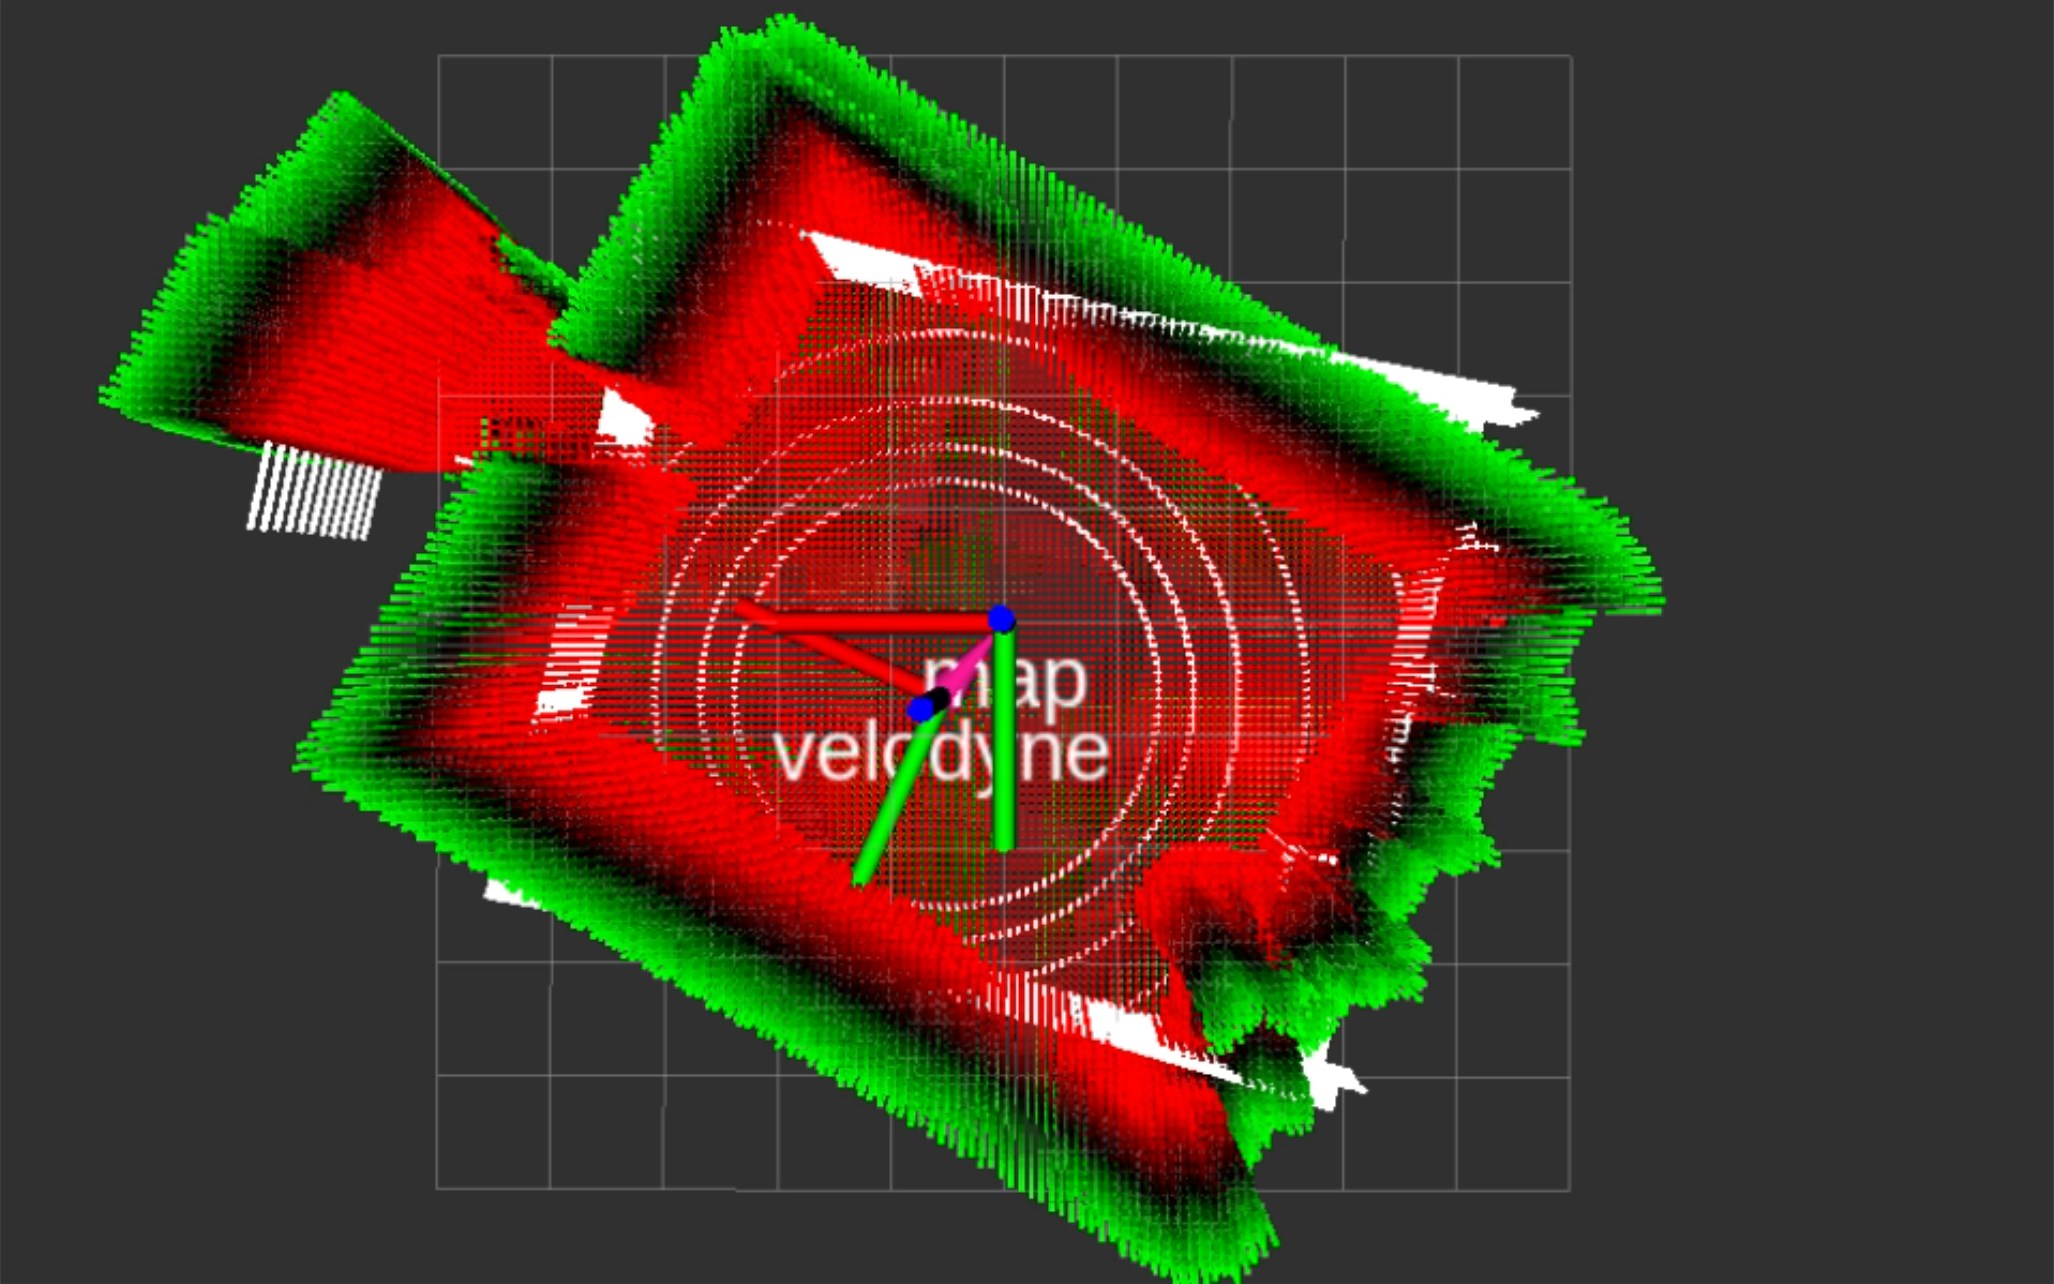
\includegraphics[width=\linewidth]{images/demo1.jpg}
\endminipage\hfill
\minipage{0.49\textwidth}
    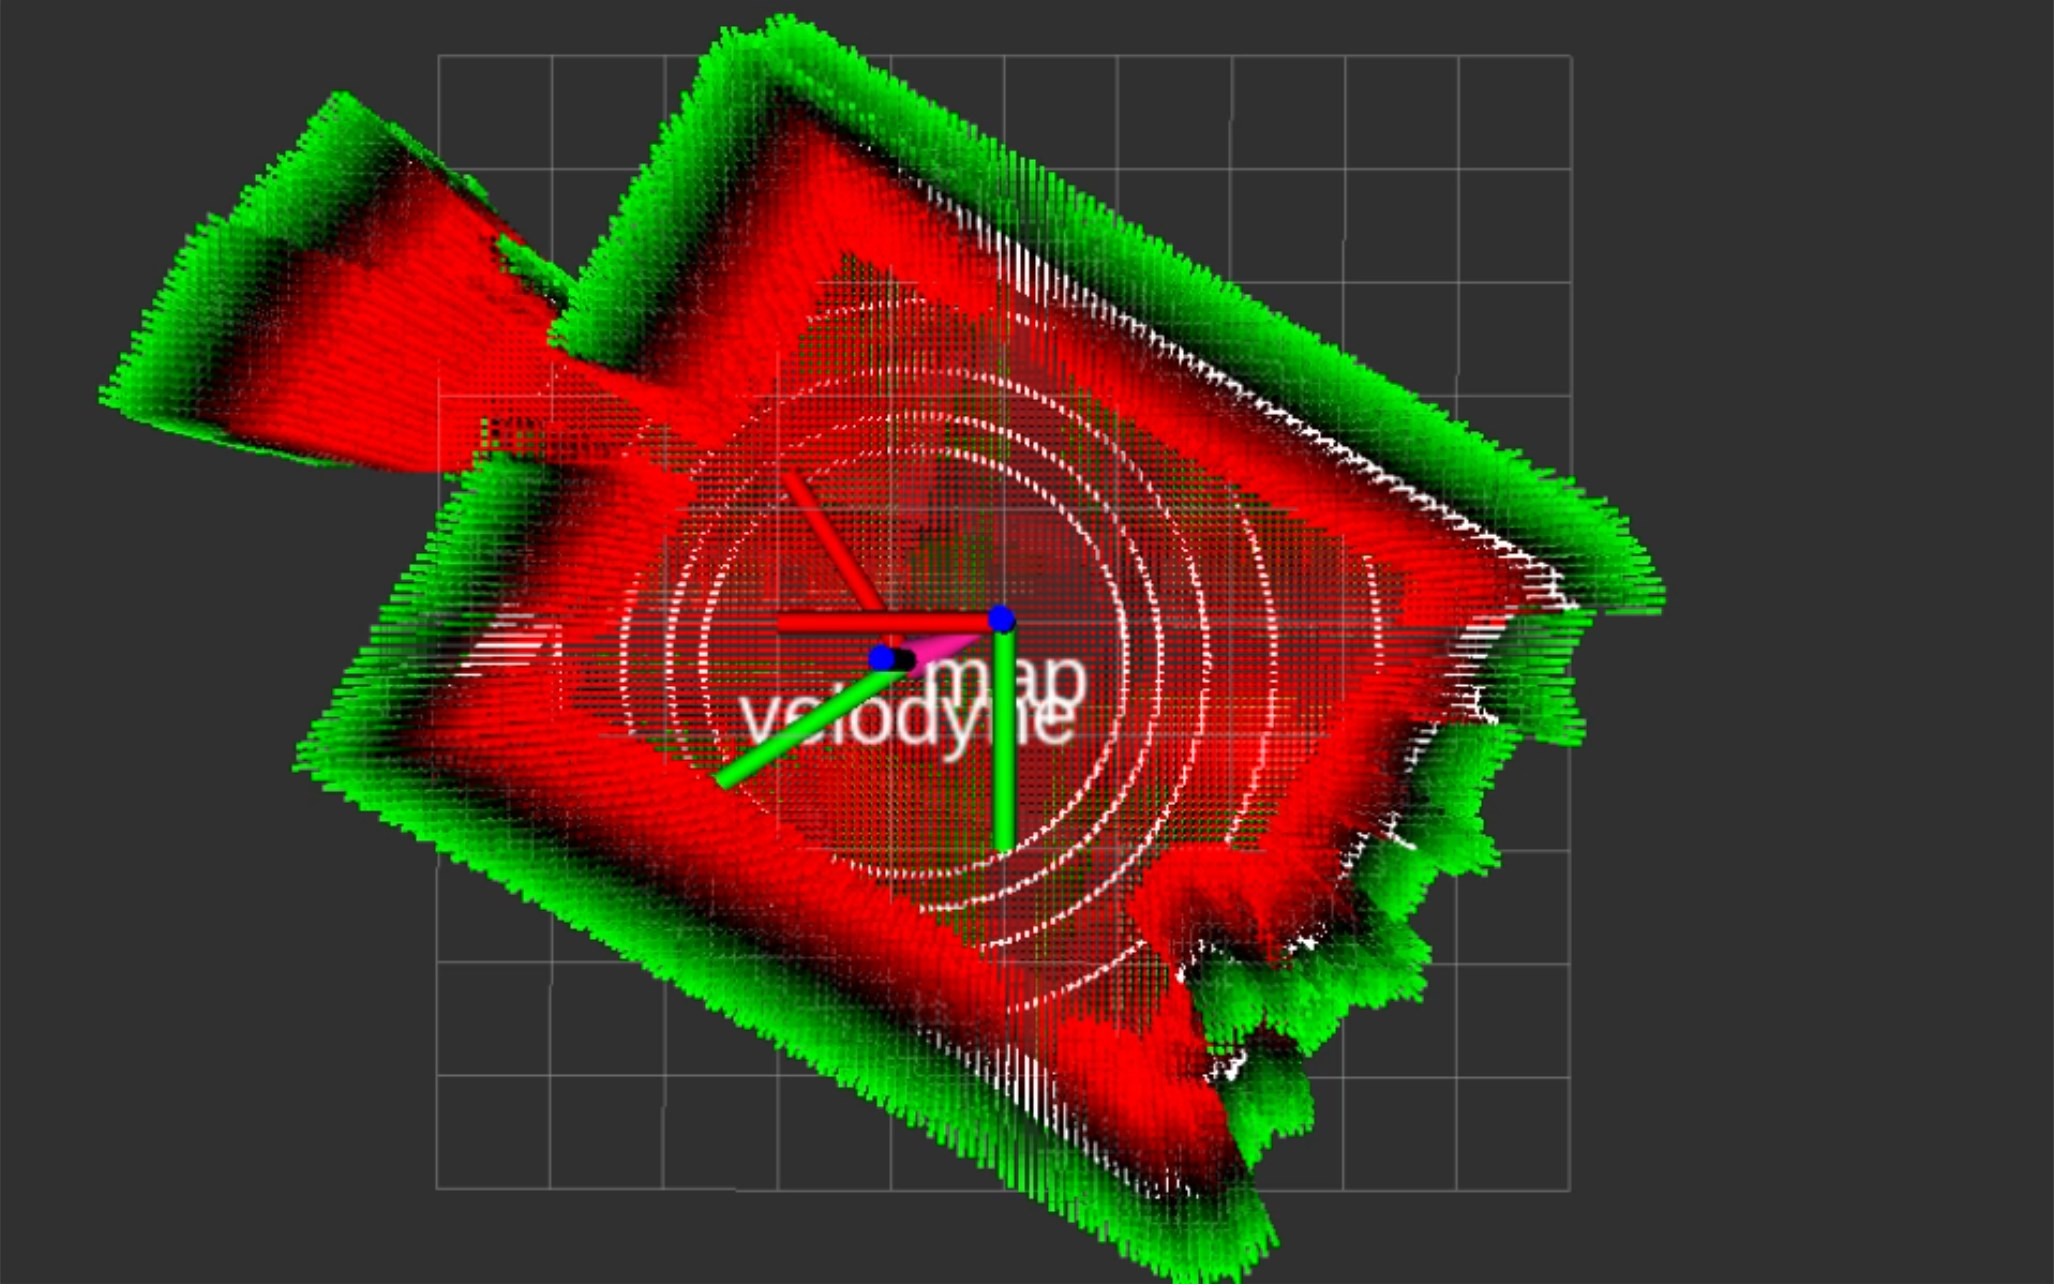
\includegraphics[width=\linewidth]{images/demo2.jpg}
\endminipage\hfill
\end{figure}
\end{frame}

\subsection{Algorithmus}
\begin{frame}{\subsecname}
\begin{center}
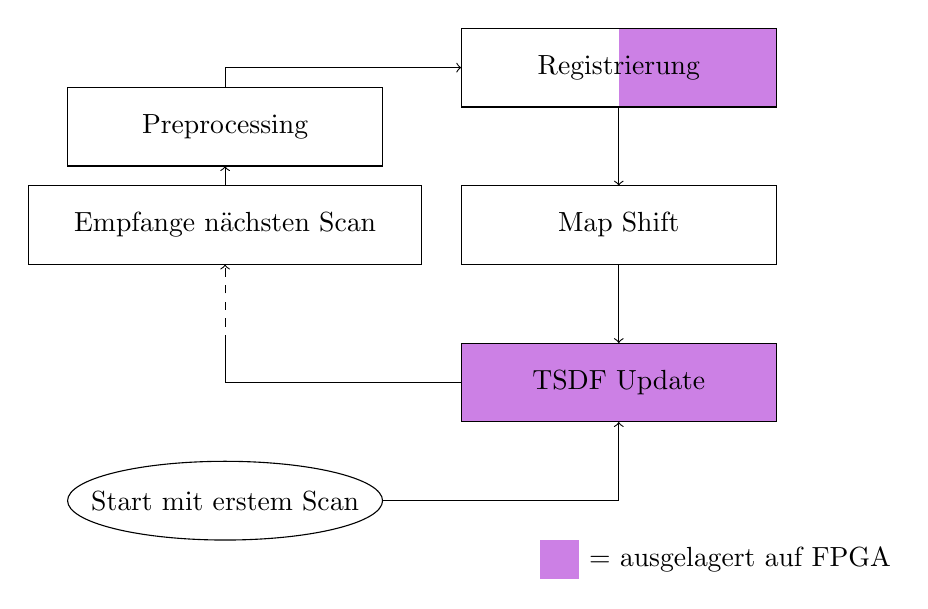
\begin{tikzpicture}
\fill [fpga] (2, 4) rectangle +(2, 1);
\draw (0, 4) rectangle +(4, 1);
\node at (2, 4.5) {Registrierung};
\draw [->] (2, 4) -- (2, 3);
\draw (0, 2) rectangle +(4, 1);
\node at (2, 2.5) {Map Shift};
\draw [->] (2, 2) -- (2, 1);
\draw [fill=fpga] (0, 0) rectangle +(4, 1);
\node at (2, 0.5) {TSDF Update};
\draw (0, 0.5) -- (-3, 0.5) -- (-3, 1);
\draw [->, dashed] (-3, 1) -- (-3, 2);
\draw (-5.5, 2) rectangle +(5, 1);
\node at (-3, 2.5) {Empfange nächsten Scan};
\draw [->] (-3, 3) -- (-3, 3.25);
\draw (-5, 3.25) rectangle +(4, 1);
\node at (-3, 3.75) {Preprocessing};
\draw [->] (-3, 4.25) -- (-3, 4.5) -- (0, 4.5);
\draw (-3, -1) ellipse (2cm and 0.5cm) node{Start mit erstem Scan};
\draw [->] (-1, -1) -- (2, -1) -- (2, 0);

\fill [fpga] (1, -2) rectangle +(0.5, 0.5);
\node [right] at (1.5, -1.75) {= ausgelagert auf FPGA};
\end{tikzpicture}
\end{center}
\end{frame}

\begin{frame}{\subsecname}
\begin{center}
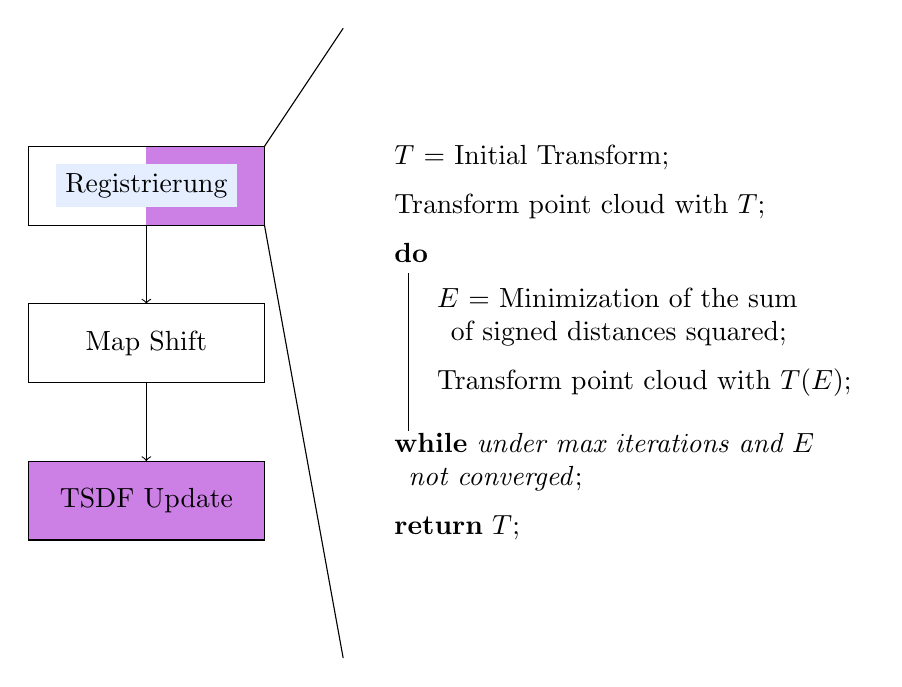
\begin{tikzpicture}
\fill [fpga] (1.5, 4) rectangle +(1.5, 1);
\draw (0, 4) rectangle +(3, 1);
\node [fill=light] at (1.5, 4.5) {Registrierung};
\draw [->] (1.5, 4) -- (1.5, 3);
\draw (0, 2) rectangle +(3, 1);
\node at (1.5, 2.5) {Map Shift};
\draw [->] (1.5, 2) -- (1.5, 1);
\draw [fill=fpga] (0, 0) rectangle +(3, 1);
\node at (1.5, 0.5) {TSDF Update};
\draw (3, 5) -- (4, 6.5);
\draw (3, 4) -- (4, -1.5);
\node [right] at (4, 2.5) {\begin{minipage}{6.5cm}
\begin{algorithm}[H]
\SetKwRepeat{Do}{do}{while}
$T$ = Initial Transform\;
\vspace{0.2cm}
Transform point cloud with $T$\;
\vspace{0.2cm}
\Do{under max iterations and $E$ not converged}{
    \vspace{0.2cm}
    $E$ = Minimization of the sum of signed distances squared\;
    \vspace{0.2cm}
    \mbox{Transform point cloud with $T(E)$\;}
    \vspace{0.1cm}
}
\vspace{0.2cm}
\Return $T$\;
\end{algorithm}
\end{minipage}};
\end{tikzpicture}
\end{center}

\begin{textblock*}{1cm}(5.5cm,4.3cm)

\begin{tikzpicture}
\draw [ultra thick, fpga] (0, 0) rectangle (6, 2);
\end{tikzpicture}
\end{textblock*}
\end{frame}

\begin{frame}{\subsecname}
\begin{center}
\begin{tikzpicture}
\fill [fpga] (1.5, 4) rectangle +(1.5, 1);
\draw (0, 4) rectangle +(3, 1);
\node at (1.5, 4.5) {Registrierung};
\draw [->] (1.5, 4) -- (1.5, 3);
\draw (0, 2) rectangle +(3, 1);
\node [fill=light] at (1.5, 2.5) {Map Shift};
\draw [->] (1.5, 2) -- (1.5, 1);
\draw [fill=fpga] (0, 0) rectangle +(3, 1);
\node at (1.5, 0.5) {TSDF Update};
\draw (3, 3) -- (4, 6.5);
\draw (3, 2) -- (4, -1.5);
\node [right] at (4, 2.5) {\begin{minipage}{6.5cm}
\begin{itemize}
\item{LocalMap (aka RingBuffer)}
\begin{itemize}
\item{Geteilt zwischen SW und HW}
\end{itemize}
\end{itemize}
\definecolor{cyan}{rgb}{0, 1, 1}
\begin{tabular}{ccc}
\begin{tikzpicture}[scale=0.125]
\node at (-1.1, 8) {
\includegraphics[width=2cm]{images/mario.png}};
\draw (0, 0) grid (16, 16);
\draw[ultra thick, cyan] (9, 9) rectangle +(5, 5);
\end{tikzpicture}
\hspace{-0.5cm}
&
\begin{tikzpicture}[scale=0.125]
\node at (-1.1, 8) {
\includegraphics[width=2cm]{images/mario.png}};
\draw (0, 0) grid (16, 16);
\draw[thick, cyan, dashed] (9, 9) rectangle +(5, 5);
\draw[ultra thick, cyan] (9, 6) rectangle +(5, 5);
\end{tikzpicture}
\hspace{-0.5cm}
&
\begin{tikzpicture}[scale=0.125]
\node at (-1.1, 8) {
\includegraphics[width=2cm]{images/mario.png}};
\draw (0, 0) grid (16, 16);
\draw[thick, cyan, dashed] (9, 9) rectangle +(5, 5);
\draw[thick, cyan, dashed] (9, 6) rectangle +(5, 5);
\draw[ultra thick, cyan] (6, 6) rectangle +(5, 5);
\end{tikzpicture}
\hspace{-0.5cm}
\\
\begin{tikzpicture}[scale=0.125]
\node at (-1.1, 2.5) {
\includegraphics[width=0.625cm]{images/a.png}};
\draw (0, 0) grid (5, 5);
\end{tikzpicture}
\hspace{-0.5cm}
&
\begin{tikzpicture}[scale=0.125]
\node at (-1.1, 2.5) {
\includegraphics[width=0.625cm]{images/b.png}};
\draw (0, 0) grid (5, 5);
\draw[ultra thick, cyan] (0, 2) -- (5, 2);
\end{tikzpicture}
\hspace{-0.5cm}
&
\begin{tikzpicture}[scale=0.125]
\node at (-1.1, 2.5) {
\includegraphics[width=0.625cm]{images/c.png}};
\draw (0, 0) grid (5, 5);
\draw[ultra thick, cyan] (0, 2) -- (5, 2);
\draw[ultra thick, cyan] (2, 0) -- (2, 5);
\end{tikzpicture}
\hspace{-0.5cm}
\\
\end{tabular}
\begin{itemize}
\item{Werte außerhalb in GlobalMap}
\begin{itemize}
\item{Chunk-basiert}
\end{itemize}
\item{Speicherung in HDF5}
\end{itemize}
\end{minipage}};
\end{tikzpicture}
\end{center}
\end{frame}

\begin{frame}{\subsecname}
\begin{center}
\begin{tikzpicture}
\fill [fpga] (1.5, 4) rectangle +(1.5, 1);
\draw (0, 4) rectangle +(3, 1);
\node at (1.5, 4.5) {Registrierung};
\draw [->] (1.5, 4) -- (1.5, 3);
\draw (0, 2) rectangle +(3, 1);
\node at (1.5, 2.5) {Map Shift};
\draw [->] (1.5, 2) -- (1.5, 1);
\draw [fill=fpga] (0, 0) rectangle +(3, 1);
\node [fill=light] at (1.5, 0.5) {TSDF Update};
\draw (3, 1) -- (4, 6.5);
\draw (3, 0) -- (4, -1.5);
\node [right] at (4, 2.5) {\begin{minipage}{6.5cm}
\begin{itemize}
\item[1.]{TSDF Generierung\\
\mbox{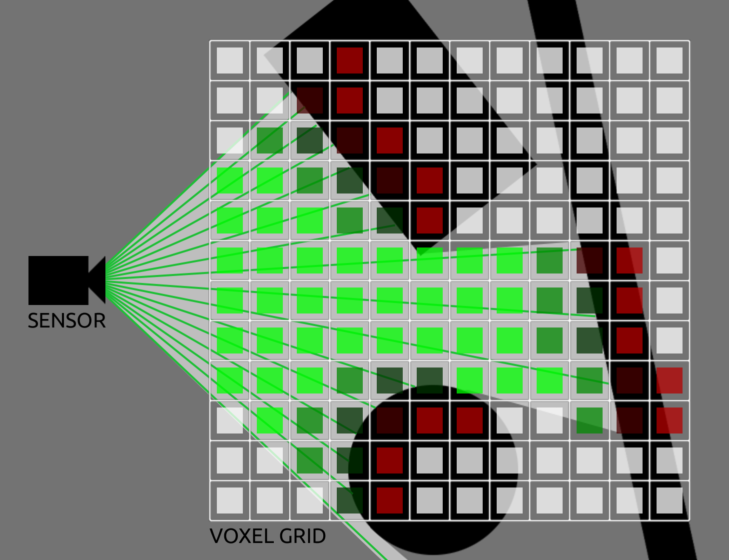
\includegraphics[height=2.8cm]{images/tsdf_calc.png}\hspace{0.1cm}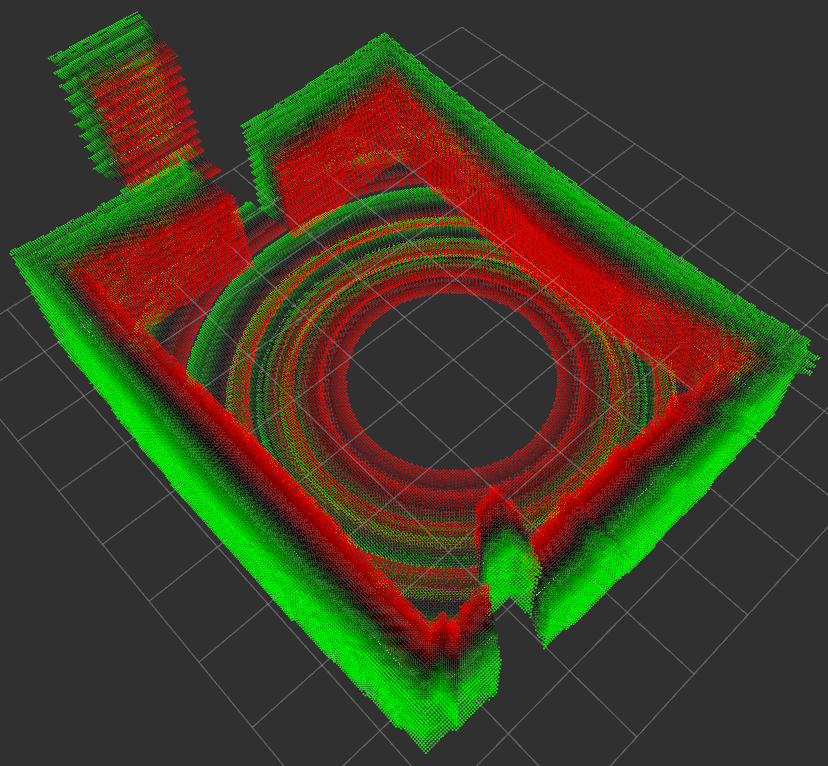
\includegraphics[height=2.8cm]{images/tsdf_map.png}}\\
\begin{footnotesize}\hspace{1.75cm}\cite{sdf_tracker}\end{footnotesize}}
\item[2.]{Update mit gewichtetem Mittelwert
\begin{align*}
M_V &= \frac{M_V \cdot M_W + v \cdot w}{M_W + w} \\
M_W &= \min(M_W + w, W_{\text{max}})
\end{align*}}
\end{itemize}
\end{minipage}};
\end{tikzpicture}
\end{center}
\end{frame}

%\subsection{Hardware Implementierung}
%\begin{frame}{\subsecname}
%\begin{center}
%\begin{LARGE}
%Registrierung
%\end{LARGE}
%\end{center}
%begin{itemize}
%\item{Parallelisierbare Schritte der Schleife in HW\\(Berechnungen für alle Punkte)}
%\item{Matrixinvertierung in der Schleife bleibt in SW}
%\end{itemize}
%\vspace{1cm}
%\begin{center}
%\begin{LARGE}
%TSDF Update
%\end{LARGE}
%\end{center}
%\begin{itemize}
%\item{Vollständig in HW}
%\item{Bresenham Algorithmus für die Iteration über Punkte entlang eines Strahls}
%\item{Synchronisation angepasst}
%\end{itemize}
%\end{frame}

\subsection{Aufbau Demo}
\begin{frame}{\subsecname}
\begin{center}
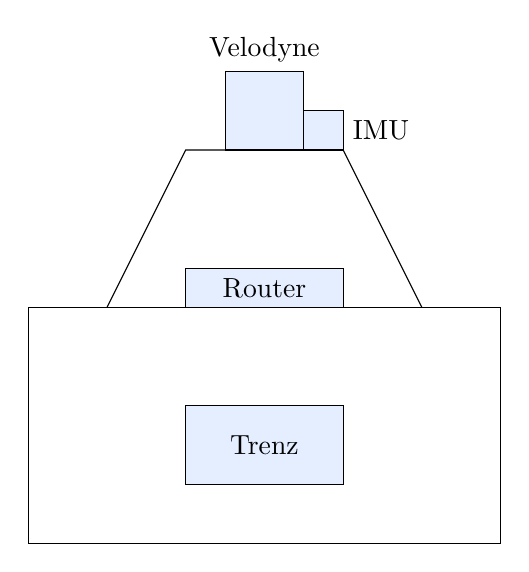
\begin{tikzpicture}
\draw (0, 0) rectangle (6, 3);
\draw (1, 3) -- (2, 5) -- (4, 5) -- (5, 3);
\draw [fill=light] (2, 0.75) rectangle +(2, 1);
\node at (3, 1.25) {Trenz};
\draw [fill=light] (2, 3) rectangle +(2, 0.5);
\node at (3, 3.25) {Router};
\draw [fill=light] (2.5, 5) rectangle +(1, 1);
\node [above] at (3, 6) {Velodyne};
\draw [fill=light] (3.5, 5) rectangle +(0.5, 0.5);
\node [right] at (4, 5.25) {IMU};
\end{tikzpicture}
\end{center}
\end{frame}

\begin{frame}{\subsecname}
\begin{center}
\begin{tabular}{cc}
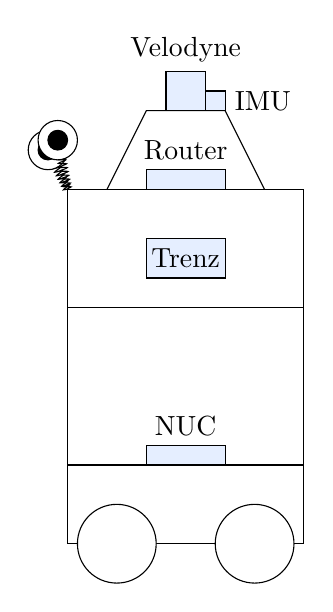
\begin{tikzpicture}[scale=0.5]
\draw (0, 0) rectangle (6, 3);
\draw (1, 3) -- (2, 5) -- (4, 5) -- (5, 3);
\draw [fill=light] (2, 0.75) rectangle +(2, 1);
\node at (3, 1.25) {Trenz};
\draw [fill=light] (2, 3) rectangle +(2, 0.5);
\node [above] at (3, 3.5) {Router};
\draw [fill=light] (2.5, 5) rectangle +(1, 1);
\node [above] at (3, 6) {Velodyne};
\draw (0, 0) -- (0, -6) -- (6, -6) -- (6, 0);
\draw [fill=light] (3.5, 5) rectangle +(0.5, 0.5);
\node [right] at (4, 5.25) {IMU};
\draw (0, -4) -- (6, -4);
\draw [fill=light] (2, -4) rectangle +(2, 0.5);
\node [above] at (3, -3.5) {NUC};
%\draw [fill=light] (2.5, -6) rectangle +(1, 0.5);
%\node [above] at (3, -5.5) {IMU};
\draw [fill=white] (1.25, -6) circle (1);
\draw [fill=white] (4.75, -6) circle (1);
\draw [decorate, decoration={snake, segment length=0.5mm, amplitude=0.5mm}] (-0.5, 4) -- (0, 3);
\draw [fill=white] (-0.5, 4) circle (0.5);
\draw [fill=black] (-0.5, 4) circle (0.25);
\draw [decorate, decoration={snake, segment length=0.5mm, amplitude=0.5mm}] (-0.25, 4.25) -- (0, 3);
\draw [fill=white] (-0.25, 4.25) circle (0.5);
\draw [fill=black] (-0.25, 4.25) circle (0.25);
\end{tikzpicture} &
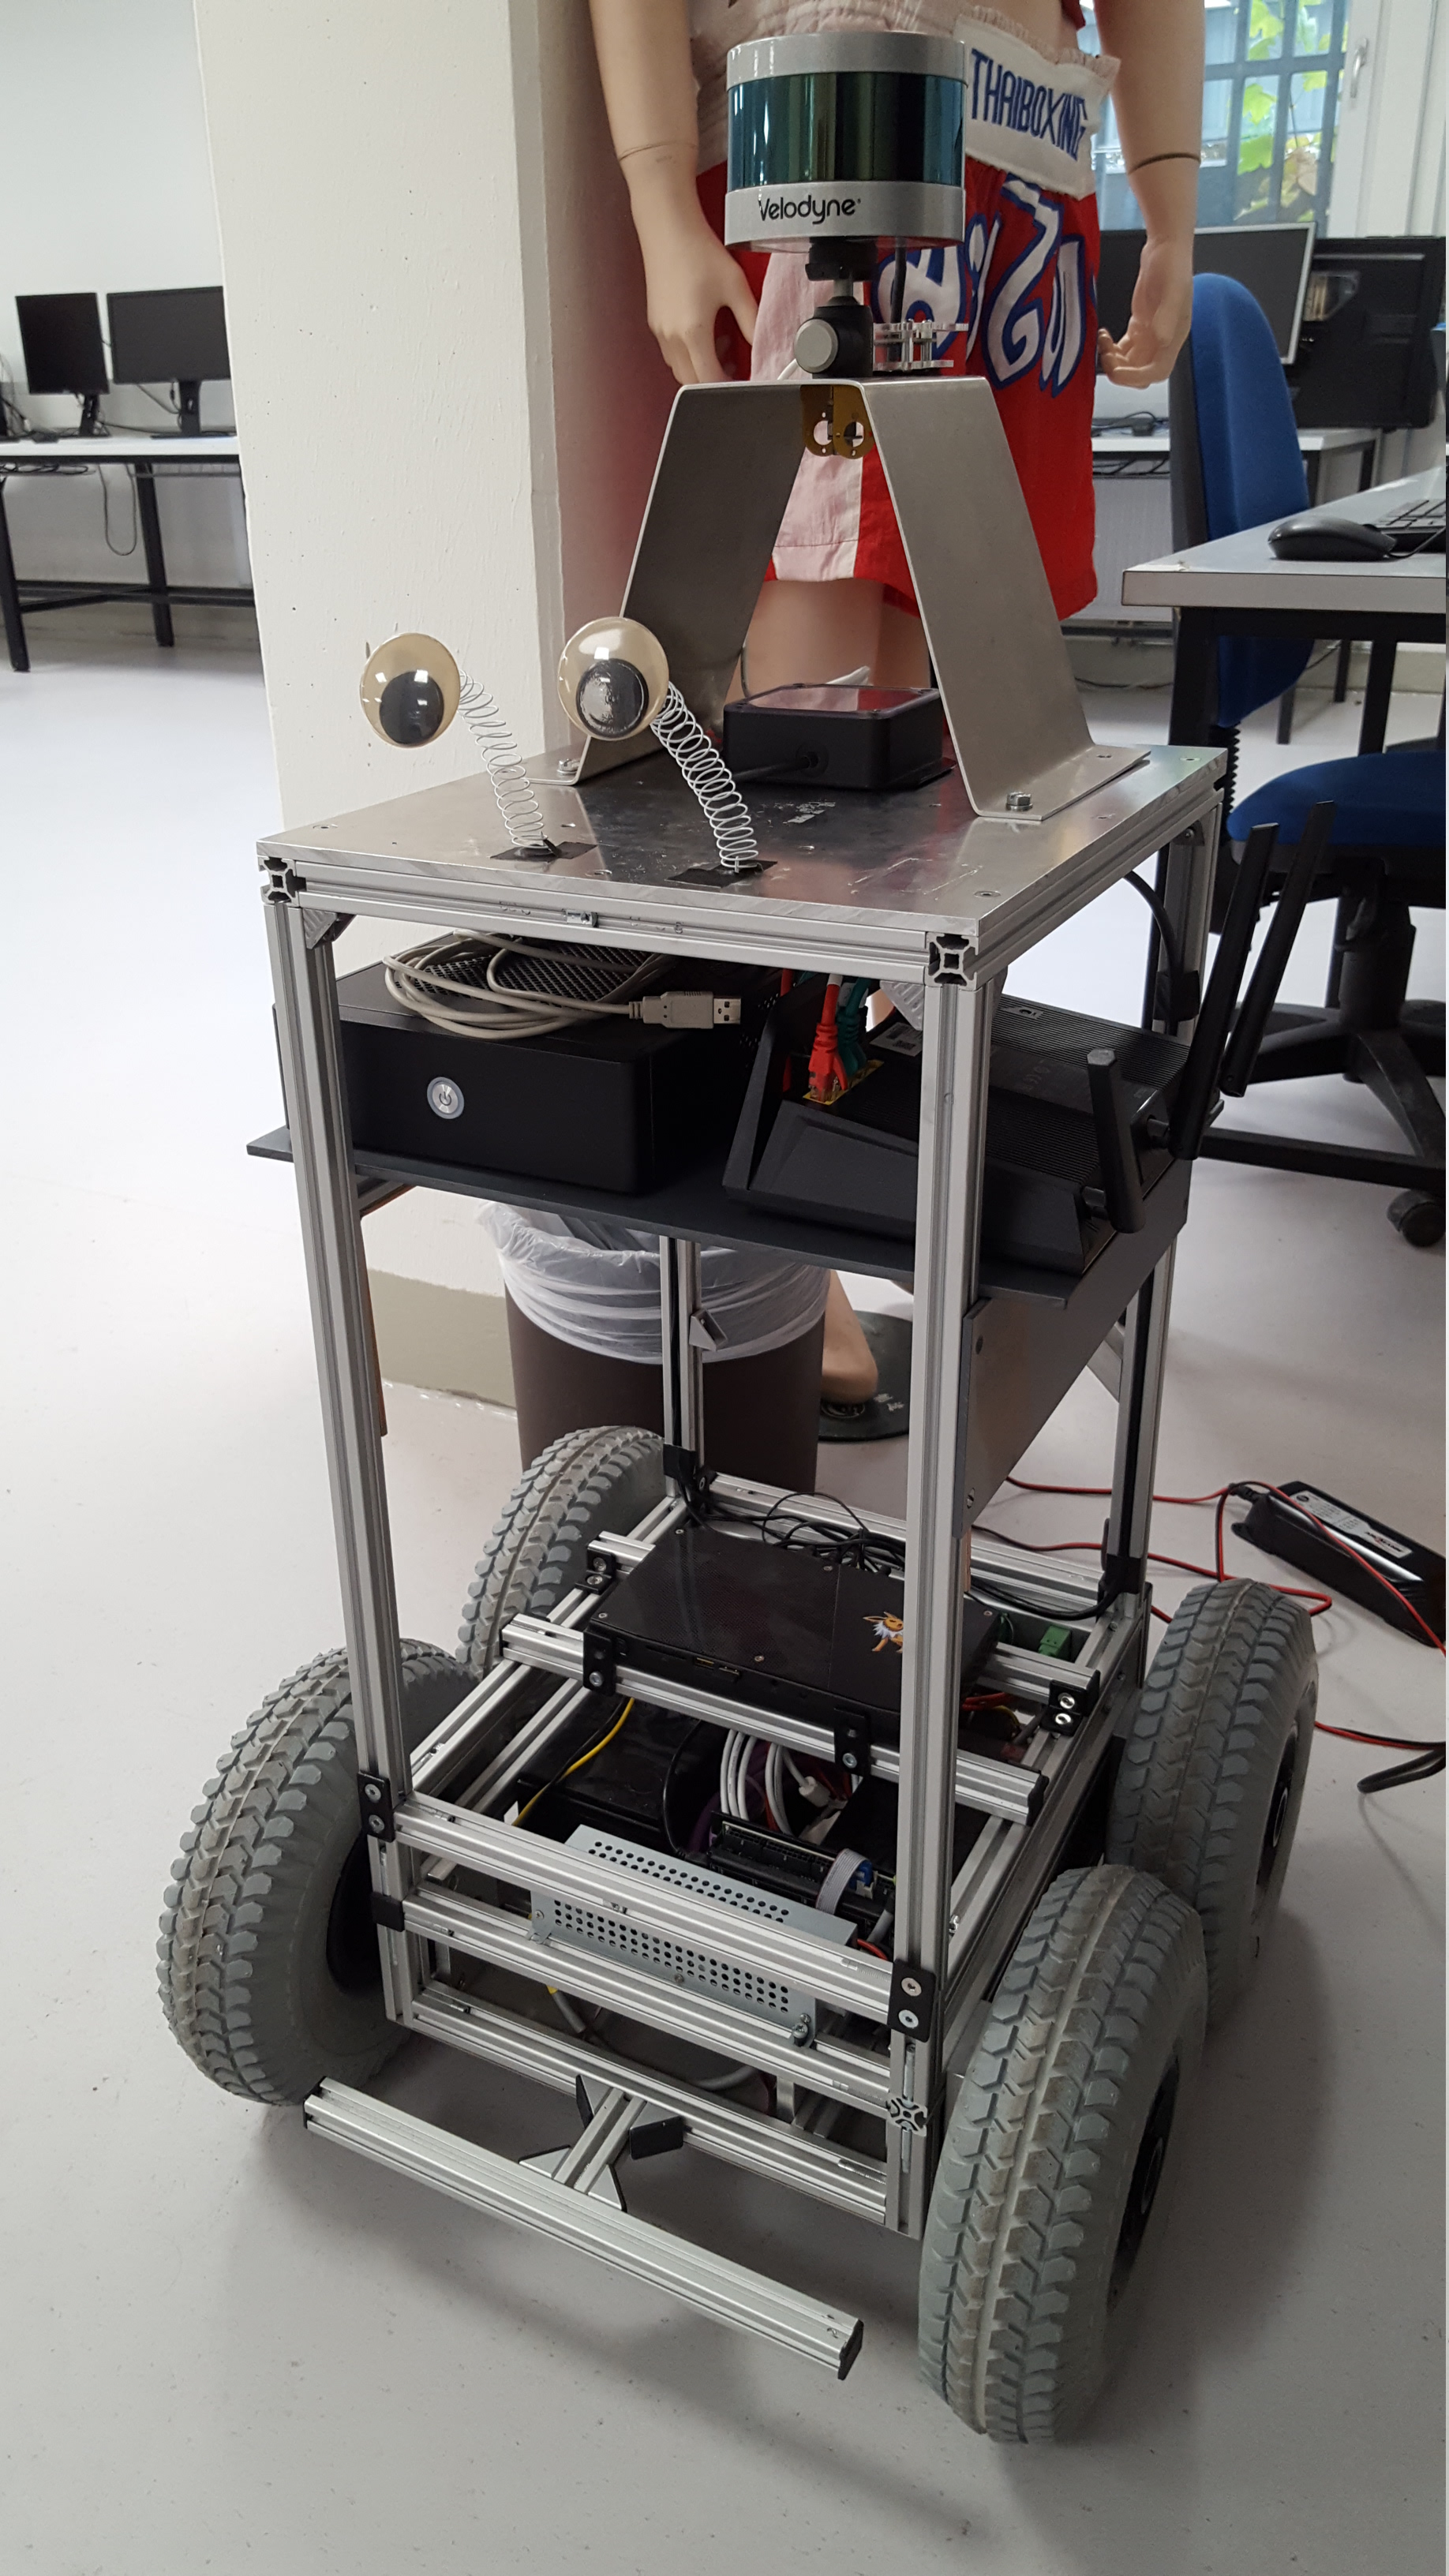
\includegraphics[height=8cm]{images/robot.jpg}
\end{tabular}
\end{center}
\end{frame}

\subsection{Kommunikation}
\begin{frame}{\subsecname}
\begin{itemize}
\item Kommunikation via \glqq{}Bridge\grqq{}%:\\Schnittstelle zwischen Sensordaten / berechneten Daten auf Trenz Board und einem Host Computer mit ROS
\item Datenaustausch uber TCP, basierend auf ZeroMQ
%\begin{itemize}
%\item LAN: Nahe real time TODO evaluieren 
%\item WLAN: TODO test mit ballermann WLAN empfaenger und ordentlichem Router
%\end{itemize}
\end{itemize}
%\item Ermoeglicht
%\begin{itemize}
%\item Visualisierung und Ueberpruefung von IMU Rohdaten, TSDF Werte, PointCloud mit ROS Tools 
%\item Aufnahme aller (oder mancher) Daten zur spaeteren Verarbeitung und Evaluation fuer einen mobilen Roboter
%\end{itemize}
\begin{center}
\begin{tikzpicture}[scale=0.3]
\draw (0, 0) rectangle (6, 3);
\draw (1, 3) -- (2, 5) -- (4, 5) -- (5, 3);
\draw [fill=light] (2, 0.75) rectangle +(2, 1);
%\node at (3, 1.25) {Trenz};
\draw [fill=light] (2, 3) rectangle +(2, 0.5);
\node [left] at (1.5, 3.75) {Router};
\draw [fill=light] (2.5, 5) rectangle +(1, 1);
%\node [above] at (3, 6) {Velodyne};
\draw (0, 0) -- (0, -6) -- (6, -6) -- (6, 0);
\draw [fill=light] (2, 5) rectangle +(0.5, 0.5);
%\node [right] at (4, 5.25) {IMU};
\draw (0, -4) -- (6, -4);
\draw [fill=light] (2, -4) rectangle +(2, 0.5);
%\node [above] at (3, -3.5) {NUC};
%\draw [fill=light] (2.5, -6) rectangle +(1, 0.5);
%\node [above] at (3, -5.5) {IMU};
\draw [fill=white] (1.25, -6) circle (1);
\draw [fill=white] (4.75, -6) circle (1);
\draw [decorate, decoration={snake, segment length=0.5mm, amplitude=0.5mm}] (6.5, 4) -- (6, 3);
\draw [fill=white] (6.5, 4) circle (0.5);
\draw [fill=black] (6.5, 4) circle (0.25);
\draw [decorate, decoration={snake, segment length=0.5mm, amplitude=0.5mm}] (6.25, 4.25) -- (6, 3);
\draw [fill=white] (6.25, 4.25) circle (0.5);
\draw [fill=black] (6.25, 4.25) circle (0.25);

\draw (18, 2) rectangle +(6, 4);
\node at (21, 4) {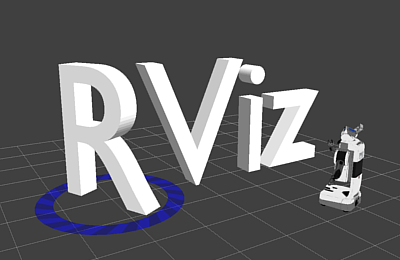
\includegraphics[height=1.05cm]{images/rviz.png}};
\draw (18.25, 2.25) rectangle +(5.5, 3.5);
\draw [fill=light] (16, 1.25) rectangle +(1.5, 4);
\draw (20.75, 2) -- (20.75, 1.5) -- (20, 1.5) -- (20, 1.25) -- (22, 1.25) -- (22, 1.5) -- (21.25, 1.5) -- (21.25, 2);
\draw (18.5, 0) -- (23.5, 0) -- (23, 0.5) -- (19, 0.5) -- cycle;

\draw [<->] (8, 3.25) -- (14, 3.25);

\node [below] at (11, 3) {\begin{minipage}{2cm}
\begin{itemize}
\item{IMU}
\item{PCL}
\item{Map}
\end{itemize}
\end{minipage}};
\end{tikzpicture}
\end{center}
\end{frame}



\section{Evaluation}
\begin{frame}{}
\begin{center}

\begin{tikzpicture}
\fill[light] (0, 0) rectangle (8, 2);
\node[dark] at (4, 1) {\begin{LARGE}\secname\end{LARGE}};
\end{tikzpicture}
\end{center}
\end{frame}

\subsection{Strom}
\begin{frame}{\subsecname}
\begin{center}

\includegraphics[width=7cm]{images/strom_rl-produktiv.png}

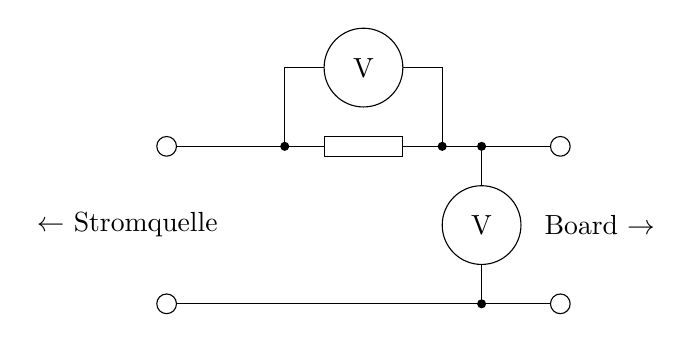
\begin{tikzpicture}[scale=0.5]
\draw (0, 0) circle (0.25);
\draw (0, 4) circle (0.25);
\draw (10, 0) circle (0.25);
\draw (10, 4) circle (0.25);
\draw (0.25, 0) -- (9.75, 0);
\draw (0.25, 4) -- (9.75, 4);
\draw (3, 4) -- (3, 6) -- (7, 6) -- (7, 4);
\draw (8, 0) -- (8, 4);
\draw [fill=black] (3, 4) circle (0.1);
\draw [fill=black] (7, 4) circle (0.1);
\draw [fill=black] (8, 0) circle (0.1);
\draw [fill=black] (8, 4) circle (0.1);
\draw [fill=white] (5, 6) circle (1) node{V};
\draw [fill=white] (8, 2) circle (1) node{V};
\draw [fill=white] (4, 3.75) rectangle (6, 4.25);
\node at (-1, 2) {$\leftarrow$ Stromquelle};
\node at (11, 2) {Board $\rightarrow$};
\end{tikzpicture}

\end{center}
\end{frame}

\begin{frame}{\subsecname}
TODO: Ergebnisse
\end{frame}

\subsection{Zeit}
\begin{frame}{\subsecname}
\centering
\begin{tabular}{ |p{3cm}||p{2cm}|p{2cm}|p{2cm}|  }
 \hline
 \multicolumn{4}{|c|}{Zeitmessung [ms]} \\
 \hline
 Abschnitt      & Durchschnitt &  Min &  Max \\
 \hline
 Preprocessing  &           35 &   24 &   51 \\
 Registrierung  &          676 &  142 & 2894 \\
 Map Shift      &          105 &    0 & 1681 \\
 TSDF Update    &          337 &  319 &  346 \\
 \hline
\end{tabular}
\end{frame}

\begin{frame}{\subsecname}
\centering
\begin{tabular}{ |l||l|l|  }
 \hline
 \multicolumn{3}{|c|}{Vergleich Vitis -- Realität [ms]} \\
 \hline
 Abschnitt      & Vitis & Gemessen\\
 \hline
 Registrierung  & 0.905 & 3.667 \\
 TSDF Update    & 124.483 & 552.924 \\
 \hline
\end{tabular}
\begin{itemize}
\item{Bei der Registrierung wird die meiste Zeit auf Speicher gewartet (95\%)}
\end{itemize}
\end{frame}

\begin{frame}{\subsecname}
\centering
\begin{tabular}{ |p{3cm}||p{2cm}|p{2cm}|p{2cm}|  }
 \hline
 \multicolumn{4}{|c|}{Vergleich verschiedener Plattformen [ms]} \\
 \hline
 Programm       & FastSense & Prototyp & Prototyp \\
 \hline
 System         &     Board &    NUC   & Stand-PC \\
 \hline
 Preprocessing  &        35 &      ??? &      ??? \\
 Registrierung  &       676 &      ??? &      ??? \\
 Map Shift      &       105 &      ??? &      ??? \\
 TSDF Update    &       337 &      ??? &      ??? \\
\hline
\end{tabular}
\end{frame}



\section{Fazit}
\begin{frame}{}
\begin{center}

\begin{tikzpicture}
\fill[light] (0, 0) rectangle (8, 2);
\node[dark] at (4, 1) {\begin{LARGE}\secname\end{LARGE}};
\end{tikzpicture}
\end{center}
\end{frame}

%\subsection{Bisherige Verbesserungen}
%\begin{frame}{\subsecname}
%\begin{itemize}
%\item{Registrierung}
%\begin{itemize}
%\item{Auslagerung von Point to TSDF auf Hardware}
%\item{Auslagerung von Pointcloud Transformation auf Hardware}
%\end{itemize}
%\item{TSDF}
%\end{itemize}
%\end{frame}

\subsection{Verbesserungspotenzial}
\begin{frame}{\subsecname}
\begin{itemize}
\item{Registrierung}
\begin{itemize}
\item{Drift entfernen (aktuell 1cm/s in alle 3 Richtungen)}
\item{Komplett in Hardware (Overhead ist fast dreimal so hoch wie der eigentliche Aufruf)}
\item{Registrierung hat Probleme mit Bresenham-Approximation der TSDF-Werte}
\begin{itemize}
\item{Stabilisierung durch trilineare Interpolation}
\end{itemize}
\end{itemize}
\item{TSDF}
\begin{itemize}
\item{Alternative zum Bresenham Algorithmus}
\begin{itemize}
\item{Voraussetzung: Effiziente Umsetzbarkeit in Hardware}
\end{itemize}
\end{itemize}
\end{itemize}
\end{frame}

\subsection{Projektmanagement}
\begin{frame}{\subsecname}
\begin{textblock*}{12.7cm}(0cm,1cm)
\begin{center}
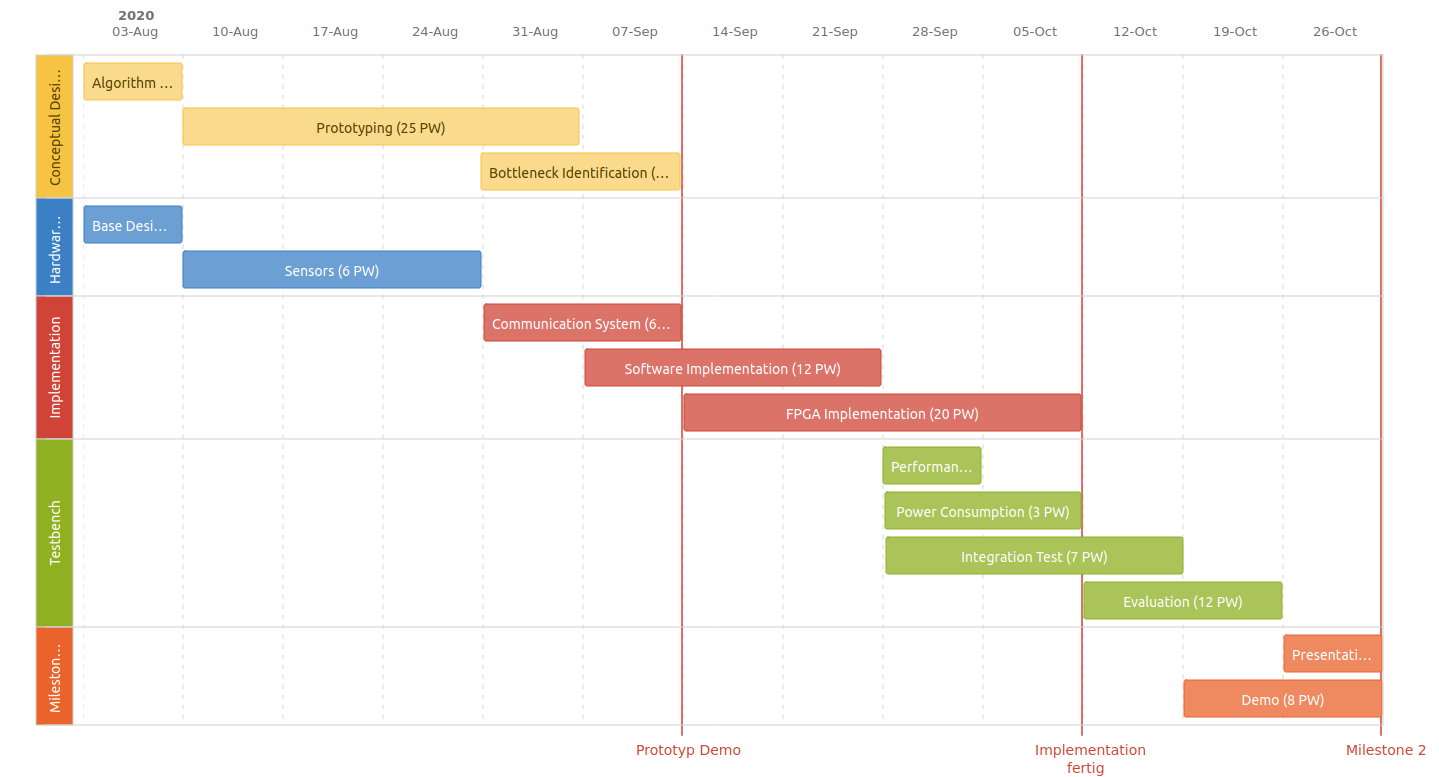
\includegraphics[width=12cm]{images/roadmap.png}
\end{center}
\end{textblock*}
\end{frame}

\begin{frame}{\subsecname}
\begin{textblock*}{12.7cm}(0cm,1cm)
\begin{center}
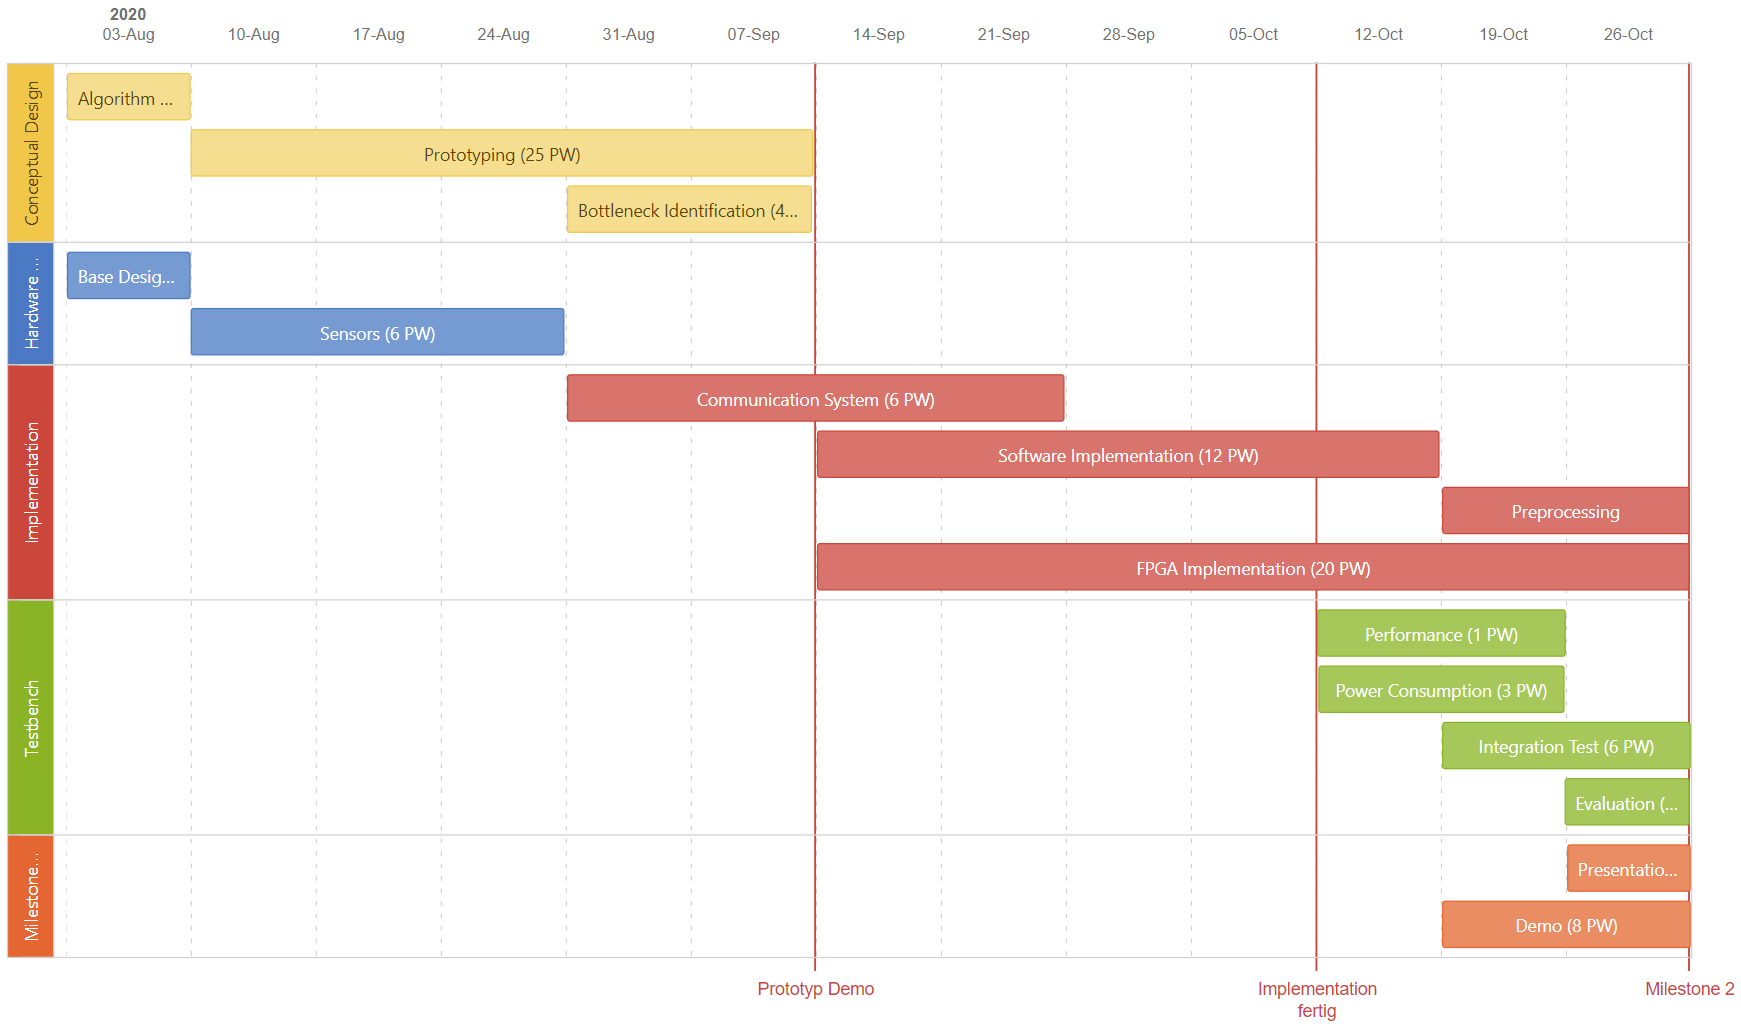
\includegraphics[width=12cm]{images/roadmap_new.png}
\end{center}
\end{textblock*}
\end{frame}

\section{Ausblick / MS3}
\begin{frame}{\secname}
\begin{itemize}
\item{Aufbau einer SLAM-Box mittels CAD}
\begin{itemize}
\item{Nutzung als Sensor}
\item{Einfache Portierung zwischen Drohne, Roboter, Rucksack etc.}
\item{Festes Interface, einfache Bedienung, Kapselung}
\end{itemize}
\item{Verbesserung und Optimierung des Algorithmus}
\item{Mesh-Generierung auf Basis der TSDF Werte}
\item{Loop Closing}
\item{Integrierung von GPS}
\end{itemize}
\end{frame}

\begin{frame}{Quellen}
\printbibliography{}
\end{frame}

\end{document}
